% -------------------------------------
% -- Assignment 1: Cooling of Coffee --
% -- Math 3090 ------------------------

% Set document type
\documentclass[11pt,oneside]{extarticle}


\usepackage{amsmath}
\usepackage{amssymb}
\usepackage{amsthm}
%\usepackage{thmtools}
\usepackage{fontspec}
\usepackage[margin=0.5in]{geometry}
\usepackage{inputenc}
%\usepackage{unicode-math}
\usepackage{setspace}
\usepackage{fancyhdr}
\usepackage{garamondx}
\usepackage{graphicx}
\usepackage{hyperref}
\usepackage{float}
\usepackage{listings}
\usepackage{newtxmath}
\usepackage{gensymb}
\usepackage{solarized-light}
\usepackage{xcolor}
%\usepackage{lmodern}

%\usepackage[default]{sourcecodepro}
\usepackage[T1]{fontenc}
%\usepackage{inconsolata}
% Real number symbol
\newcommand{\Real}{\mathbb{R}}
\newcommand{\dprime}{{\prime\prime}}
\newcommand{\Celsius}{\:\degree\mathrm{C}}
\newcommand{\Dollar}{\$}
\newcommand{\percent}{\%}
%\newcommand{\min}{\mathrm{min}\:}

% Set typewriter font to Source Code Pro
%\renewcommand{\ttfamily}{\tiny\sourcecodepro}

% Change enumerator to use letters i.e., a, b, c, ...
\renewcommand{\theenumi}{\alph{enumi}}

\renewcommand{\eqref}[1]{\textup{\emph{({\ref*{#1}})}}}
\numberwithin{equation}{section}
\numberwithin{figure}{section}

\setlength{\belowcaptionskip}{-12pt}
%\setttfont{

% Set paragraph indent to 0cm
\setlength{\parindent}{0cm}
%\setlength{\parskip}{1cm plus4mm minus3mm}
\setlength{\parskip}{0.25cm}

\begin{document}

\section{Changing room temperature}

\par Modify the coffee model to account for a room temperature that starts at $20\Celsius$,
and increases at a constant rate to a maximum $26\Celsius$ in $2$ hours, and then
stays at the maximum temperature. Assume that the initial temperature of the cofee
is $100\Celsius$ and after $10$ minutes, the temperature of the coffee is $90\Celsius$.
Modify the codes and draw the room temperature and coffee temperature in the same
diagram for $6$ hours.

\subsection{Building model}

\par The independent variable of the model is time $t$ in hours. The observed temperature
of the coffee $u_{obs}(t)$ is a function of time, with units$\Celsius$.

\par Let $u_{sur}$ be the surruounding temperature, then $u_{sur}$ is given by

\begin{equation}
    u_{sur}(t) = 
    \begin{cases} 
        20 + 3t & 0 \leq t \leq 2 \\
        26 & t > 2 \\
    \end{cases}.
\end{equation}

\par We use the model presented in class, but modify it to use $u_{sur}(t)$ to
get 

\begin{equation}
    \frac{du}{dt}
    =
    c(u_{sur}(t)-u)
\end{equation}

Now, we discretize the model with the timestep $h=\Delta t$ to get

\begin{equation}
    \frac{u_{k+1} - u_k}{h}
    =
    hc(u_{sur}(t_k) - u_k)
\end{equation}

where $t_k = k\Delta t$ is the discrete time, at the $k^{th}$ step. This is the
Newton Forward method.

\subsection{Result}

\begin{figure}[H]
    \caption{Coffee in room with changing temperature}
    \label{fig:analytic}
    \begin{center}
        {\graphicspath{{./figures/}}
        % GNUPLOT: LaTeX picture with Postscript
\begingroup
  \makeatletter
  \providecommand\color[2][]{%
    \GenericError{(gnuplot) \space\space\space\@spaces}{%
      Package color not loaded in conjunction with
      terminal option `colourtext'%
    }{See the gnuplot documentation for explanation.%
    }{Either use 'blacktext' in gnuplot or load the package
      color.sty in LaTeX.}%
    \renewcommand\color[2][]{}%
  }%
  \providecommand\includegraphics[2][]{%
    \GenericError{(gnuplot) \space\space\space\@spaces}{%
      Package graphicx or graphics not loaded%
    }{See the gnuplot documentation for explanation.%
    }{The gnuplot epslatex terminal needs graphicx.sty or graphics.sty.}%
    \renewcommand\includegraphics[2][]{}%
  }%
  \providecommand\rotatebox[2]{#2}%
  \@ifundefined{ifGPcolor}{%
    \newif\ifGPcolor
    \GPcolortrue
  }{}%
  \@ifundefined{ifGPblacktext}{%
    \newif\ifGPblacktext
    \GPblacktexttrue
  }{}%
  % define a \g@addto@macro without @ in the name:
  \let\gplgaddtomacro\g@addto@macro
  % define empty templates for all commands taking text:
  \gdef\gplbacktext{}%
  \gdef\gplfronttext{}%
  \makeatother
  \ifGPblacktext
    % no textcolor at all
    \def\colorrgb#1{}%
    \def\colorgray#1{}%
  \else
    % gray or color?
    \ifGPcolor
      \def\colorrgb#1{\color[rgb]{#1}}%
      \def\colorgray#1{\color[gray]{#1}}%
      \expandafter\def\csname LTw\endcsname{\color{white}}%
      \expandafter\def\csname LTb\endcsname{\color{black}}%
      \expandafter\def\csname LTa\endcsname{\color{black}}%
      \expandafter\def\csname LT0\endcsname{\color[rgb]{1,0,0}}%
      \expandafter\def\csname LT1\endcsname{\color[rgb]{0,1,0}}%
      \expandafter\def\csname LT2\endcsname{\color[rgb]{0,0,1}}%
      \expandafter\def\csname LT3\endcsname{\color[rgb]{1,0,1}}%
      \expandafter\def\csname LT4\endcsname{\color[rgb]{0,1,1}}%
      \expandafter\def\csname LT5\endcsname{\color[rgb]{1,1,0}}%
      \expandafter\def\csname LT6\endcsname{\color[rgb]{0,0,0}}%
      \expandafter\def\csname LT7\endcsname{\color[rgb]{1,0.3,0}}%
      \expandafter\def\csname LT8\endcsname{\color[rgb]{0.5,0.5,0.5}}%
    \else
      % gray
      \def\colorrgb#1{\color{black}}%
      \def\colorgray#1{\color[gray]{#1}}%
      \expandafter\def\csname LTw\endcsname{\color{white}}%
      \expandafter\def\csname LTb\endcsname{\color{black}}%
      \expandafter\def\csname LTa\endcsname{\color{black}}%
      \expandafter\def\csname LT0\endcsname{\color{black}}%
      \expandafter\def\csname LT1\endcsname{\color{black}}%
      \expandafter\def\csname LT2\endcsname{\color{black}}%
      \expandafter\def\csname LT3\endcsname{\color{black}}%
      \expandafter\def\csname LT4\endcsname{\color{black}}%
      \expandafter\def\csname LT5\endcsname{\color{black}}%
      \expandafter\def\csname LT6\endcsname{\color{black}}%
      \expandafter\def\csname LT7\endcsname{\color{black}}%
      \expandafter\def\csname LT8\endcsname{\color{black}}%
    \fi
  \fi
    \setlength{\unitlength}{0.0500bp}%
    \ifx\gptboxheight\undefined%
      \newlength{\gptboxheight}%
      \newlength{\gptboxwidth}%
      \newsavebox{\gptboxtext}%
    \fi%
    \setlength{\fboxrule}{0.5pt}%
    \setlength{\fboxsep}{1pt}%
\begin{picture}(7200.00,5040.00)%
    \gplgaddtomacro\gplbacktext{%
      \csname LTb\endcsname%%
      \put(814,704){\makebox(0,0)[r]{\strut{}$20$}}%
      \put(814,1188){\makebox(0,0)[r]{\strut{}$30$}}%
      \put(814,1672){\makebox(0,0)[r]{\strut{}$40$}}%
      \put(814,2156){\makebox(0,0)[r]{\strut{}$50$}}%
      \put(814,2640){\makebox(0,0)[r]{\strut{}$60$}}%
      \put(814,3125){\makebox(0,0)[r]{\strut{}$70$}}%
      \put(814,3609){\makebox(0,0)[r]{\strut{}$80$}}%
      \put(814,4093){\makebox(0,0)[r]{\strut{}$90$}}%
      \put(814,4577){\makebox(0,0)[r]{\strut{}$100$}}%
      \put(946,484){\makebox(0,0){\strut{}$0$}}%
      \put(1759,484){\makebox(0,0){\strut{}$50$}}%
      \put(2573,484){\makebox(0,0){\strut{}$100$}}%
      \put(3386,484){\makebox(0,0){\strut{}$150$}}%
      \put(4200,484){\makebox(0,0){\strut{}$200$}}%
      \put(5013,484){\makebox(0,0){\strut{}$250$}}%
      \put(5827,484){\makebox(0,0){\strut{}$300$}}%
      \put(6640,484){\makebox(0,0){\strut{}$350$}}%
    }%
    \gplgaddtomacro\gplfronttext{%
      \csname LTb\endcsname%%
      \put(198,2761){\rotatebox{-270}{\makebox(0,0){\strut{}Temperature (Degrees C)}}}%
      \put(3874,154){\makebox(0,0){\strut{}Time $t$ (minutes)}}%
      \csname LTb\endcsname%%
      \put(5816,4646){\makebox(0,0)[r]{\strut{}Room temp. $u_{sur}(t)$}}%
      \csname LTb\endcsname%%
      \put(5816,4426){\makebox(0,0)[r]{\strut{}Coffee temp. $u(t)$}}%
    }%
    \gplbacktext
    \put(0,0){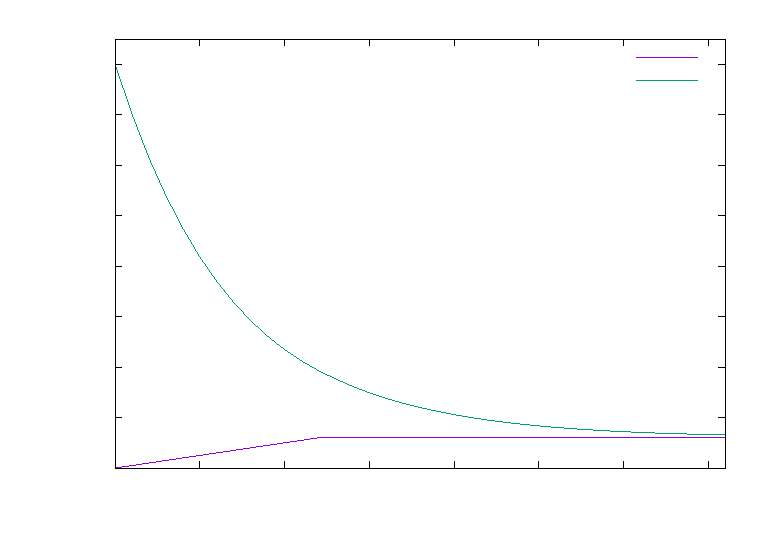
\includegraphics{/home/jacques/repos/math3090/assignments/assignment1/figures/figure1-1}}%
    \gplfronttext
  \end{picture}%
\endgroup
} 
        
        \scriptsize{ {\bf Description:} The analytic solution $U(t)$ plotted for $\rho = 0.1$,
        $u_{m} = 6\Celsius$, and $t^* = 50$ minutes. The disconuity is clearly visible when
        the milk is added to the coffee. The horizontal line shows $u_d$. The intersection
        of the lines is when $U(t)=u_d$.}
    \end{center}
\end{figure}

\newpage

\section{When to add milk?}

\par Do you add the milk to coffee straight away? People often ask wheter it is better
to add the cold milk to a hot cup of coffee straight away or wait for a while to
let it cool down and then add the cold milk.

\par Estimate the optimal time to add cold milk so that the coffee cools down to
the drinkable temperature fastests. Let us assume that the drinable temperature
is $50\Celsius$. Assume that the initial temperature of the coffee is $100\Celsius$
and the insulation of the cup is $0.01282$. Room temperature is fixed at $22\Celsius$.
Is your result reasonable? Explain it briefly. Based on your result, make suggestion
to the people about when to add coffee.


\par You can use and modify the model and codes we developed in the class for the
cooling of the coffee in a constant room temperature. Assume that the temperature
of the coffee is independent on special variables. Make further assumptions if needed.

\subsection{Preliminary discussion and assumptions}

\par A realistic physical treatment of the problem of mixing disimilar fluids at
different temperatures is an enormously complicated problem. Simulating such a
scenario requires both accurate $3D$ spacial fluid simulation coupled with a 
thermal dynamic simulation.

\par Instead of dealing with the complexity of mixing fluids we will confine
ourselves to some simplifications. All physical properties of the liquids
(asside from temperature) are taken to be identical. Mixing the milk into the
coffee causes an instantaneous change temperature. The only factors we consider
are the temperature of the milk $u_{milk}^{(i)}$ before mixing, and the ratio of the mass
of the milk divided by the mass of the coffee $\rho$ given by

\subsection{Model}

\begin{equation}
    \frac{dU}{dt} = c( u_{sur} - U) \quad\text{for}\quad t \neq t^*.
\end{equation}

\begin{equation}
    \label{eq:model2}
    U(t) = 
    \begin{cases} 
        u(t)                &   t < t^* \\
        u_{mix}             & t = t^* \\
        v(t)                &   t > t^* \\
    \end{cases}.
\end{equation}

\begin{equation}
    \frac{du}{dt} = c(u_{sur} - u)\quad\text{for}\quad t < t^*,
    \quad\text{with}\quad
    u(0) = U(0) = u_0 
\end{equation}

\begin{equation}
    \frac{dv}{dt} = c(u_{sur} - v)\quad\text{for}\quad t > t^*
    \quad\text{with}\quad
    v(t^*) = v_0 = u_{mix}
\end{equation}

\begin{equation}
    \label{eq:mix}
    T = \frac{m_1T_1 + m_2T_2}{m_1+m_2}
    =
    \frac{m_1(T_1 + \rho T_2)}{m_1(1+\rho)}
    =
    \frac{ T_1 + \rho T_2 }{ 1 + \rho },
    \quad\text{where}\quad
    \rho = \frac{m_2}{m_1}
\end{equation}

Taking \eqref{eq:mix}, with $T_1 = u(t^*)$, and the milk temperature $u_m$ we can get $u_{mix}$,

\begin{equation}
    u_{mix} = 
    v_0 = v(t^*) =
    \frac{ u(t^*) + \rho u_m }{ 1 + \rho }
\end{equation}

\subsection{Analytical model}

We can easily find a closed form solution for $U(t)$ by solving the constrained
differential equation \eqref{eq:model2}.

\begin{equation}
    \alpha(t) = \alpha_0 e^{-ct}
    \quad\text{and}\quad
    \beta(t) = \beta_0 e^{-c(t - t^*)}
\end{equation}

where $\alpha(t) = u(t) - u_{sur}$ and $\beta(t) = v(t) - u_{sur}$, with intial
conditions $\alpha_0 = \alpha(0) = u_0 - u_{sur}$ and $\beta_0 = \beta(t^*) =
v_0 - u_{sur}$. The closed form solution is then

\begin{equation}
    \label{eq:model2-analytic}
    U(t) =
    \begin{cases}
        \alpha_0e^{-ct} + u_{sur}   &   t < t^* \\
        \beta_0e^{-c(t-t^*)} + u_{sur}  & t \geq t^* \\
    \end{cases}
\end{equation}


\begin{figure}[H]
    \caption{Analytical solution}
    \label{fig:analytic}
    \begin{center}
        {\graphicspath{{./figures/}}
        % GNUPLOT: LaTeX picture with Postscript
\begingroup
  \makeatletter
  \providecommand\color[2][]{%
    \GenericError{(gnuplot) \space\space\space\@spaces}{%
      Package color not loaded in conjunction with
      terminal option `colourtext'%
    }{See the gnuplot documentation for explanation.%
    }{Either use 'blacktext' in gnuplot or load the package
      color.sty in LaTeX.}%
    \renewcommand\color[2][]{}%
  }%
  \providecommand\includegraphics[2][]{%
    \GenericError{(gnuplot) \space\space\space\@spaces}{%
      Package graphicx or graphics not loaded%
    }{See the gnuplot documentation for explanation.%
    }{The gnuplot epslatex terminal needs graphicx.sty or graphics.sty.}%
    \renewcommand\includegraphics[2][]{}%
  }%
  \providecommand\rotatebox[2]{#2}%
  \@ifundefined{ifGPcolor}{%
    \newif\ifGPcolor
    \GPcolortrue
  }{}%
  \@ifundefined{ifGPblacktext}{%
    \newif\ifGPblacktext
    \GPblacktexttrue
  }{}%
  % define a \g@addto@macro without @ in the name:
  \let\gplgaddtomacro\g@addto@macro
  % define empty templates for all commands taking text:
  \gdef\gplbacktext{}%
  \gdef\gplfronttext{}%
  \makeatother
  \ifGPblacktext
    % no textcolor at all
    \def\colorrgb#1{}%
    \def\colorgray#1{}%
  \else
    % gray or color?
    \ifGPcolor
      \def\colorrgb#1{\color[rgb]{#1}}%
      \def\colorgray#1{\color[gray]{#1}}%
      \expandafter\def\csname LTw\endcsname{\color{white}}%
      \expandafter\def\csname LTb\endcsname{\color{black}}%
      \expandafter\def\csname LTa\endcsname{\color{black}}%
      \expandafter\def\csname LT0\endcsname{\color[rgb]{1,0,0}}%
      \expandafter\def\csname LT1\endcsname{\color[rgb]{0,1,0}}%
      \expandafter\def\csname LT2\endcsname{\color[rgb]{0,0,1}}%
      \expandafter\def\csname LT3\endcsname{\color[rgb]{1,0,1}}%
      \expandafter\def\csname LT4\endcsname{\color[rgb]{0,1,1}}%
      \expandafter\def\csname LT5\endcsname{\color[rgb]{1,1,0}}%
      \expandafter\def\csname LT6\endcsname{\color[rgb]{0,0,0}}%
      \expandafter\def\csname LT7\endcsname{\color[rgb]{1,0.3,0}}%
      \expandafter\def\csname LT8\endcsname{\color[rgb]{0.5,0.5,0.5}}%
    \else
      % gray
      \def\colorrgb#1{\color{black}}%
      \def\colorgray#1{\color[gray]{#1}}%
      \expandafter\def\csname LTw\endcsname{\color{white}}%
      \expandafter\def\csname LTb\endcsname{\color{black}}%
      \expandafter\def\csname LTa\endcsname{\color{black}}%
      \expandafter\def\csname LT0\endcsname{\color{black}}%
      \expandafter\def\csname LT1\endcsname{\color{black}}%
      \expandafter\def\csname LT2\endcsname{\color{black}}%
      \expandafter\def\csname LT3\endcsname{\color{black}}%
      \expandafter\def\csname LT4\endcsname{\color{black}}%
      \expandafter\def\csname LT5\endcsname{\color{black}}%
      \expandafter\def\csname LT6\endcsname{\color{black}}%
      \expandafter\def\csname LT7\endcsname{\color{black}}%
      \expandafter\def\csname LT8\endcsname{\color{black}}%
    \fi
  \fi
    \setlength{\unitlength}{0.0500bp}%
    \ifx\gptboxheight\undefined%
      \newlength{\gptboxheight}%
      \newlength{\gptboxwidth}%
      \newsavebox{\gptboxtext}%
    \fi%
    \setlength{\fboxrule}{0.5pt}%
    \setlength{\fboxsep}{1pt}%
\begin{picture}(7200.00,5040.00)%
    \gplgaddtomacro\gplbacktext{%
      \csname LTb\endcsname%%
      \put(814,704){\makebox(0,0)[r]{\strut{}$40$}}%
      \put(814,1292){\makebox(0,0)[r]{\strut{}$50$}}%
      \put(814,1880){\makebox(0,0)[r]{\strut{}$60$}}%
      \put(814,2468){\makebox(0,0)[r]{\strut{}$70$}}%
      \put(814,3055){\makebox(0,0)[r]{\strut{}$80$}}%
      \put(814,3643){\makebox(0,0)[r]{\strut{}$90$}}%
      \put(814,4231){\makebox(0,0)[r]{\strut{}$100$}}%
      \put(814,4819){\makebox(0,0)[r]{\strut{}$110$}}%
      \put(946,484){\makebox(0,0){\strut{}$0$}}%
      \put(1922,484){\makebox(0,0){\strut{}$20$}}%
      \put(2898,484){\makebox(0,0){\strut{}$40$}}%
      \put(3875,484){\makebox(0,0){\strut{}$60$}}%
      \put(4851,484){\makebox(0,0){\strut{}$80$}}%
      \put(5827,484){\makebox(0,0){\strut{}$100$}}%
      \put(6803,484){\makebox(0,0){\strut{}$120$}}%
    }%
    \gplgaddtomacro\gplfronttext{%
      \csname LTb\endcsname%%
      \put(198,2761){\rotatebox{-270}{\makebox(0,0){\strut{}Temperature $U(t)$}}}%
      \put(3874,154){\makebox(0,0){\strut{}Time $t$ (minutes)}}%
      \csname LTb\endcsname%%
      \put(5816,4646){\makebox(0,0)[r]{\strut{}$U(t)$}}%
      \csname LTb\endcsname%%
      \put(5816,4426){\makebox(0,0)[r]{\strut{}$u_d = 50°C$}}%
    }%
    \gplbacktext
    \put(0,0){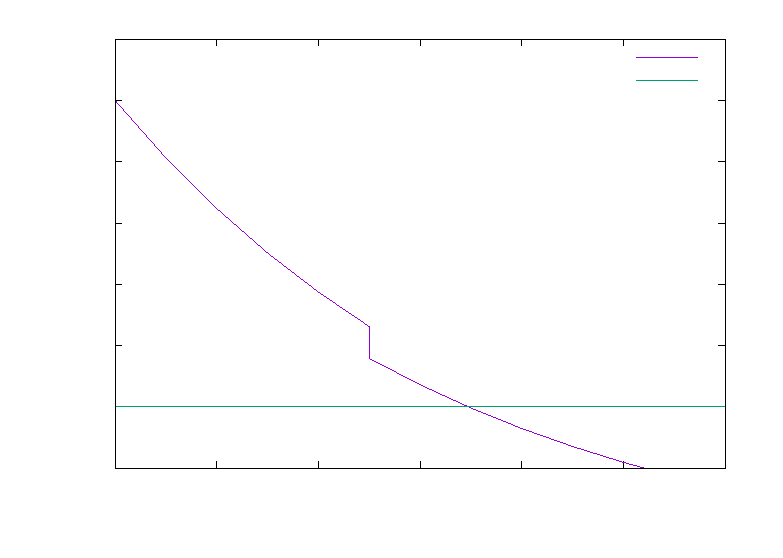
\includegraphics{/home/jacques/repos/math3090/assignments/assignment1/figures/figure2-1}}%
    \gplfronttext
  \end{picture}%
\endgroup
} 
        
        \scriptsize{ {\bf Description:} The analytic solution $U(t)$ plotted for $\rho = 0.1$,
        $u_{m} = 6\Celsius$, and $t^* = 50$ minutes. The disconuity is clearly visible when
        the milk is added to the coffee. The horizontal line shows $u_d$. The intersection
        of the lines is when $U(t)=u_d$.}
    \end{center}
\end{figure}

\newpage

\subsection{Discrete Newton Forward model}

\par It is straightforward to create a discrete model. Let $h=\Delta t$ denote
the iteration step size, and let $k\in\left\lbrace0,1,\ldots\right\rbrace$ denote 
the iteration step. The initial step is to set

$$
U_0 = u_0.
$$

\begin{equation}
    U_{k} = 
    \begin{cases}
        U_{k-1} - hc( U_{k-1} - u_{sur} ) & \text{for } hk < t^* \\
        \frac{U_{k-1} + \rho u_m}{1+\rho} & \text{for } hk \leq t^* \leq h(k+1) \\
        U_{k-1} - hc( U_{k-1} - u_{sur} ) & \text{for } hk > t^* \\
\end{cases},
\end{equation}

In practice an additional point is added at $t^*$ to better 
plot the disconuity with a vertical line. This restricts the implementation to values
of $t^*$ which satisfy $\mathtt{fmod}(t^*, h) = 0$. $\mathtt{fmod}$ is the
floating point modulus function in the \emph{C++ standard library} as defined in
the {\ttfamily<cmath>} header.

\begin{figure}[H]
    \caption{Discrete solution with varying $t^*$}
    \label{fig:analytic}
    \begin{center}
        {\graphicspath{{./figures/}}
        % GNUPLOT: LaTeX picture with Postscript
\begingroup
  \makeatletter
  \providecommand\color[2][]{%
    \GenericError{(gnuplot) \space\space\space\@spaces}{%
      Package color not loaded in conjunction with
      terminal option `colourtext'%
    }{See the gnuplot documentation for explanation.%
    }{Either use 'blacktext' in gnuplot or load the package
      color.sty in LaTeX.}%
    \renewcommand\color[2][]{}%
  }%
  \providecommand\includegraphics[2][]{%
    \GenericError{(gnuplot) \space\space\space\@spaces}{%
      Package graphicx or graphics not loaded%
    }{See the gnuplot documentation for explanation.%
    }{The gnuplot epslatex terminal needs graphicx.sty or graphics.sty.}%
    \renewcommand\includegraphics[2][]{}%
  }%
  \providecommand\rotatebox[2]{#2}%
  \@ifundefined{ifGPcolor}{%
    \newif\ifGPcolor
    \GPcolortrue
  }{}%
  \@ifundefined{ifGPblacktext}{%
    \newif\ifGPblacktext
    \GPblacktexttrue
  }{}%
  % define a \g@addto@macro without @ in the name:
  \let\gplgaddtomacro\g@addto@macro
  % define empty templates for all commands taking text:
  \gdef\gplbacktext{}%
  \gdef\gplfronttext{}%
  \makeatother
  \ifGPblacktext
    % no textcolor at all
    \def\colorrgb#1{}%
    \def\colorgray#1{}%
  \else
    % gray or color?
    \ifGPcolor
      \def\colorrgb#1{\color[rgb]{#1}}%
      \def\colorgray#1{\color[gray]{#1}}%
      \expandafter\def\csname LTw\endcsname{\color{white}}%
      \expandafter\def\csname LTb\endcsname{\color{black}}%
      \expandafter\def\csname LTa\endcsname{\color{black}}%
      \expandafter\def\csname LT0\endcsname{\color[rgb]{1,0,0}}%
      \expandafter\def\csname LT1\endcsname{\color[rgb]{0,1,0}}%
      \expandafter\def\csname LT2\endcsname{\color[rgb]{0,0,1}}%
      \expandafter\def\csname LT3\endcsname{\color[rgb]{1,0,1}}%
      \expandafter\def\csname LT4\endcsname{\color[rgb]{0,1,1}}%
      \expandafter\def\csname LT5\endcsname{\color[rgb]{1,1,0}}%
      \expandafter\def\csname LT6\endcsname{\color[rgb]{0,0,0}}%
      \expandafter\def\csname LT7\endcsname{\color[rgb]{1,0.3,0}}%
      \expandafter\def\csname LT8\endcsname{\color[rgb]{0.5,0.5,0.5}}%
    \else
      % gray
      \def\colorrgb#1{\color{black}}%
      \def\colorgray#1{\color[gray]{#1}}%
      \expandafter\def\csname LTw\endcsname{\color{white}}%
      \expandafter\def\csname LTb\endcsname{\color{black}}%
      \expandafter\def\csname LTa\endcsname{\color{black}}%
      \expandafter\def\csname LT0\endcsname{\color{black}}%
      \expandafter\def\csname LT1\endcsname{\color{black}}%
      \expandafter\def\csname LT2\endcsname{\color{black}}%
      \expandafter\def\csname LT3\endcsname{\color{black}}%
      \expandafter\def\csname LT4\endcsname{\color{black}}%
      \expandafter\def\csname LT5\endcsname{\color{black}}%
      \expandafter\def\csname LT6\endcsname{\color{black}}%
      \expandafter\def\csname LT7\endcsname{\color{black}}%
      \expandafter\def\csname LT8\endcsname{\color{black}}%
    \fi
  \fi
    \setlength{\unitlength}{0.0500bp}%
    \ifx\gptboxheight\undefined%
      \newlength{\gptboxheight}%
      \newlength{\gptboxwidth}%
      \newsavebox{\gptboxtext}%
    \fi%
    \setlength{\fboxrule}{0.5pt}%
    \setlength{\fboxsep}{1pt}%
\begin{picture}(7200.00,5040.00)%
    \gplgaddtomacro\gplbacktext{%
      \csname LTb\endcsname%%
      \put(814,704){\makebox(0,0)[r]{\strut{}$30$}}%
      \put(814,1292){\makebox(0,0)[r]{\strut{}$40$}}%
      \put(814,1880){\makebox(0,0)[r]{\strut{}$50$}}%
      \put(814,2468){\makebox(0,0)[r]{\strut{}$60$}}%
      \put(814,3055){\makebox(0,0)[r]{\strut{}$70$}}%
      \put(814,3643){\makebox(0,0)[r]{\strut{}$80$}}%
      \put(814,4231){\makebox(0,0)[r]{\strut{}$90$}}%
      \put(814,4819){\makebox(0,0)[r]{\strut{}$100$}}%
      \put(946,484){\makebox(0,0){\strut{}$0$}}%
      \put(1922,484){\makebox(0,0){\strut{}$20$}}%
      \put(2898,484){\makebox(0,0){\strut{}$40$}}%
      \put(3875,484){\makebox(0,0){\strut{}$60$}}%
      \put(4851,484){\makebox(0,0){\strut{}$80$}}%
      \put(5827,484){\makebox(0,0){\strut{}$100$}}%
      \put(6803,484){\makebox(0,0){\strut{}$120$}}%
    }%
    \gplgaddtomacro\gplfronttext{%
      \csname LTb\endcsname%%
      \put(198,2761){\rotatebox{-270}{\makebox(0,0){\strut{}Temperature $U(t)$}}}%
      \put(3874,154){\makebox(0,0){\strut{}Time $t$ (minutes)}}%
      \csname LTb\endcsname%%
      \put(5816,4646){\makebox(0,0)[r]{\strut{}$t^* = 0$ mins}}%
      \csname LTb\endcsname%%
      \put(5816,4426){\makebox(0,0)[r]{\strut{}$t^* = 10$ mins}}%
      \csname LTb\endcsname%%
      \put(5816,4206){\makebox(0,0)[r]{\strut{}$t^* = 30$ mins}}%
      \csname LTb\endcsname%%
      \put(5816,3986){\makebox(0,0)[r]{\strut{}$t^* = 40$ mins}}%
      \csname LTb\endcsname%%
      \put(5816,3766){\makebox(0,0)[r]{\strut{}$t^* = 50$ mins}}%
      \csname LTb\endcsname%%
      \put(5816,3546){\makebox(0,0)[r]{\strut{}$u_d = 50°C$}}%
    }%
    \gplbacktext
    \put(0,0){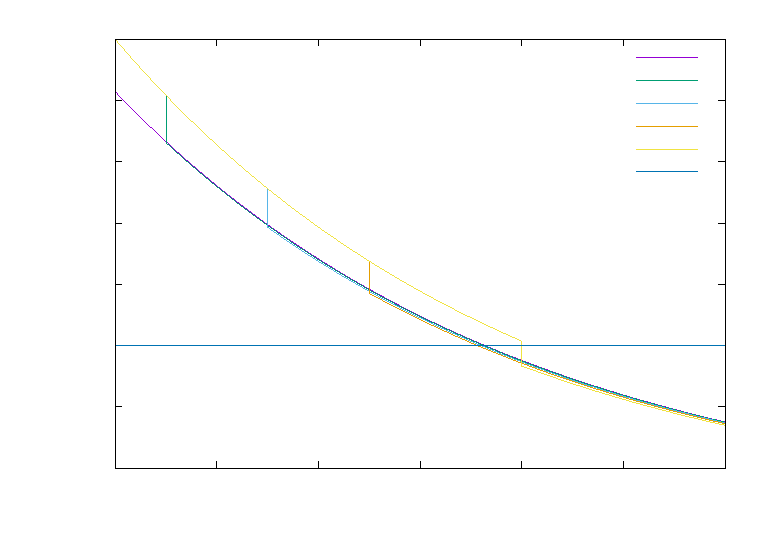
\includegraphics{/home/jacques/repos/math3090/assignments/assignment1/figures/figure2-2}}%
    \gplfronttext
  \end{picture}%
\endgroup
} 
        
        \scriptsize{ {\bf Discussion} The analytic solution $U(t)$ plotted for $\rho = 0.1$,
        $u_{m} = 6\Celsius$, and $t^* = 50$ minutes. The disconuity is clearly visible when
        the milk is added to the coffee. The horizontal line shows $u_d$. The intersection
        of the lines is when $U(t)=u_d$.}
    \end{center}
\end{figure}

% Figure 2.4 - Comparing analytical and discrete model
\begin{figure}[H]
    \caption{Comparing analytical model with discrete model for various time steps $h$}
    \label{fig:analytic}
    \begin{center}
        {\graphicspath{{./figures/}}
        % GNUPLOT: LaTeX picture with Postscript
\begingroup
  \makeatletter
  \providecommand\color[2][]{%
    \GenericError{(gnuplot) \space\space\space\@spaces}{%
      Package color not loaded in conjunction with
      terminal option `colourtext'%
    }{See the gnuplot documentation for explanation.%
    }{Either use 'blacktext' in gnuplot or load the package
      color.sty in LaTeX.}%
    \renewcommand\color[2][]{}%
  }%
  \providecommand\includegraphics[2][]{%
    \GenericError{(gnuplot) \space\space\space\@spaces}{%
      Package graphicx or graphics not loaded%
    }{See the gnuplot documentation for explanation.%
    }{The gnuplot epslatex terminal needs graphicx.sty or graphics.sty.}%
    \renewcommand\includegraphics[2][]{}%
  }%
  \providecommand\rotatebox[2]{#2}%
  \@ifundefined{ifGPcolor}{%
    \newif\ifGPcolor
    \GPcolortrue
  }{}%
  \@ifundefined{ifGPblacktext}{%
    \newif\ifGPblacktext
    \GPblacktexttrue
  }{}%
  % define a \g@addto@macro without @ in the name:
  \let\gplgaddtomacro\g@addto@macro
  % define empty templates for all commands taking text:
  \gdef\gplbacktext{}%
  \gdef\gplfronttext{}%
  \makeatother
  \ifGPblacktext
    % no textcolor at all
    \def\colorrgb#1{}%
    \def\colorgray#1{}%
  \else
    % gray or color?
    \ifGPcolor
      \def\colorrgb#1{\color[rgb]{#1}}%
      \def\colorgray#1{\color[gray]{#1}}%
      \expandafter\def\csname LTw\endcsname{\color{white}}%
      \expandafter\def\csname LTb\endcsname{\color{black}}%
      \expandafter\def\csname LTa\endcsname{\color{black}}%
      \expandafter\def\csname LT0\endcsname{\color[rgb]{1,0,0}}%
      \expandafter\def\csname LT1\endcsname{\color[rgb]{0,1,0}}%
      \expandafter\def\csname LT2\endcsname{\color[rgb]{0,0,1}}%
      \expandafter\def\csname LT3\endcsname{\color[rgb]{1,0,1}}%
      \expandafter\def\csname LT4\endcsname{\color[rgb]{0,1,1}}%
      \expandafter\def\csname LT5\endcsname{\color[rgb]{1,1,0}}%
      \expandafter\def\csname LT6\endcsname{\color[rgb]{0,0,0}}%
      \expandafter\def\csname LT7\endcsname{\color[rgb]{1,0.3,0}}%
      \expandafter\def\csname LT8\endcsname{\color[rgb]{0.5,0.5,0.5}}%
    \else
      % gray
      \def\colorrgb#1{\color{black}}%
      \def\colorgray#1{\color[gray]{#1}}%
      \expandafter\def\csname LTw\endcsname{\color{white}}%
      \expandafter\def\csname LTb\endcsname{\color{black}}%
      \expandafter\def\csname LTa\endcsname{\color{black}}%
      \expandafter\def\csname LT0\endcsname{\color{black}}%
      \expandafter\def\csname LT1\endcsname{\color{black}}%
      \expandafter\def\csname LT2\endcsname{\color{black}}%
      \expandafter\def\csname LT3\endcsname{\color{black}}%
      \expandafter\def\csname LT4\endcsname{\color{black}}%
      \expandafter\def\csname LT5\endcsname{\color{black}}%
      \expandafter\def\csname LT6\endcsname{\color{black}}%
      \expandafter\def\csname LT7\endcsname{\color{black}}%
      \expandafter\def\csname LT8\endcsname{\color{black}}%
    \fi
  \fi
    \setlength{\unitlength}{0.0500bp}%
    \ifx\gptboxheight\undefined%
      \newlength{\gptboxheight}%
      \newlength{\gptboxwidth}%
      \newsavebox{\gptboxtext}%
    \fi%
    \setlength{\fboxrule}{0.5pt}%
    \setlength{\fboxsep}{1pt}%
\begin{picture}(7200.00,5040.00)%
    \gplgaddtomacro\gplbacktext{%
      \csname LTb\endcsname%%
      \put(814,704){\makebox(0,0)[r]{\strut{}$30$}}%
      \put(814,1292){\makebox(0,0)[r]{\strut{}$40$}}%
      \put(814,1880){\makebox(0,0)[r]{\strut{}$50$}}%
      \put(814,2468){\makebox(0,0)[r]{\strut{}$60$}}%
      \put(814,3055){\makebox(0,0)[r]{\strut{}$70$}}%
      \put(814,3643){\makebox(0,0)[r]{\strut{}$80$}}%
      \put(814,4231){\makebox(0,0)[r]{\strut{}$90$}}%
      \put(814,4819){\makebox(0,0)[r]{\strut{}$100$}}%
      \put(946,484){\makebox(0,0){\strut{}$0$}}%
      \put(1922,484){\makebox(0,0){\strut{}$20$}}%
      \put(2898,484){\makebox(0,0){\strut{}$40$}}%
      \put(3875,484){\makebox(0,0){\strut{}$60$}}%
      \put(4851,484){\makebox(0,0){\strut{}$80$}}%
      \put(5827,484){\makebox(0,0){\strut{}$100$}}%
      \put(6803,484){\makebox(0,0){\strut{}$120$}}%
    }%
    \gplgaddtomacro\gplfronttext{%
      \csname LTb\endcsname%%
      \put(198,2761){\rotatebox{-270}{\makebox(0,0){\strut{}Temperature $U(t)$}}}%
      \put(3874,154){\makebox(0,0){\strut{}Time $t$ (minutes)}}%
      \csname LTb\endcsname%%
      \put(5816,4646){\makebox(0,0)[r]{\strut{}Anal. model}}%
      \csname LTb\endcsname%%
      \put(5816,4426){\makebox(0,0)[r]{\strut{}Disc. h=40.0}}%
      \csname LTb\endcsname%%
      \put(5816,4206){\makebox(0,0)[r]{\strut{}Disc. h=20.0}}%
      \csname LTb\endcsname%%
      \put(5816,3986){\makebox(0,0)[r]{\strut{}Disc. h=10.0}}%
      \csname LTb\endcsname%%
      \put(5816,3766){\makebox(0,0)[r]{\strut{}Disc. h=5.0}}%
      \csname LTb\endcsname%%
      \put(5816,3546){\makebox(0,0)[r]{\strut{}$u_d = 50°C$}}%
    }%
    \gplbacktext
    \put(0,0){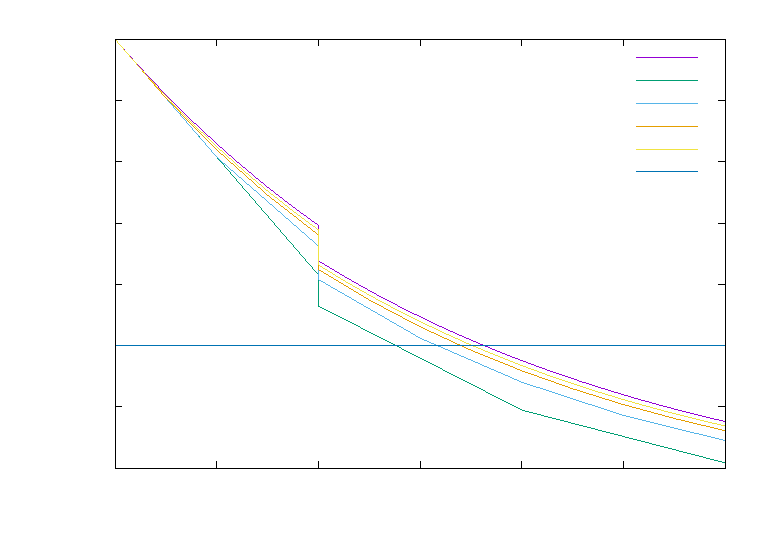
\includegraphics{/home/jacques/repos/math3090/assignments/assignment1/figures/figure2-3}}%
    \gplfronttext
  \end{picture}%
\endgroup
} 
        
        \scriptsize{ {\bf Discussion} Observe that the discrete model approaches
        the analytical solution as the time step $h$ decreases. The discretization
        step introduces a negative error into the solution. This example uses
        the following parameters values: $u_0 = 100.0\Celsius$, $u_{sur} = 22.0\Celsius$,
        $t^*=40$ mins., $\rho=0.1$, and $u_m=6.0\Celsius$.
    }
    \end{center}
\end{figure}

\subsection{Conclusions and analysis}

\par Observe that the magnitude of the first derivative of $U(t)$ decreases as 
$t\rightarrow\infty$. In order for $U(t)$ to reach $u_d$ in the minimum
amount of time, it is best to add the milk as late as possible. This maximizes
rate of the first portion of Newton cooling. Infact, the model intersects $y=u_d$,
slightly earlier as $t^*$ increases. Keep in mind that there is a limit to this.

There exists some $t_{ideal} > 0$ such that if $t^* > t_{ideal}$, adding milk to
the coffee instantly cools it below $U(t) < u_d$.

\par We can derive the optimum time $t_{ideal}$ by starting from

\begin{equation}
    u_{mix} = \frac{u(t^*) + \rho u_m }{1+\rho} = u_d = 50.0\Celsius.
\end{equation}

$$
u(t^*) = u_d(1+\rho) - \rho u_m
$$

$$
(u_0 - u_{sur})e^{-ct^*} + u_{sur} = u_d(1+\rho)-\rho u_m
$$

$$
-ct^* = \ln\left\lbrack \frac{u_d(1-\rho) - \rho u_m}{u_0 - u_{sur}}\right\rbrack
$$

\begin{equation}
    t_{ideal} = t^* = -\frac{1}{c}
    \ln\left\lbrack \frac{u_d(1-\rho) - \rho u_m}{u_0 - u_{sur}}\right\rbrack
\end{equation}

Here, $t_{ideal}$ is the latest we can add milk without cooling the coffee below
$u_d$. This minimizes the cooling time.

\newpage

% -------------------------------------
% -- Question 3 -----------------------
% -------------------------------------
\section{Compound interest}

You invest $\Dollar 100$ in a savings account paying $6\percent$ per year. Let
$y(t)$ be the amount in your account after $t$ years. If the interest rate is
compounded continuously, then $y(t)$ solves the ODE initial value problem

$$
\frac{dy}{dt} = ry
$$

where $r=6\percent=0.06$ and $y(0)=\Dollar 100$.

\begin{enumerate}

    \item What is the analytic solution $y(t)$ to this initial value problem?

        Start with the ensatz $y(t)=Ae^{rt}$, and plug into equation above.

        $$
        \frac{dy}{dt}(t) =
        rAe^{rt} = ry(t)
        $$

        Take ensatz at $t\rightarrow 0$, to determine constant $A$,
        
        $$
        y(0)=Ae^{r\cdot 0} = A
        \implies
        A = y(0) = \Dollar 100.
        $$

        The analytic solution is therefore,

        \begin{equation}
            y(t)=100e^{rt}.
            \label{eq:compound}
        \end{equation}

    \item What is the balance in your account after 10 years with each of the
        following methods of compounding interest, yearly, monthly, quarterly,
        daily, and continuous compounding?

        \par {\bf Continouos compounding} can be solved analytically using 
        \eqref{eq:compound}, as follows:

        $$
        y(10) = 100 e^{0.06\cdot 10} = \Dollar182.21.
        $$

        \par {\bf Yearly} 
        
        \par {\bf Monthly} 
        \par {\bf Quarterly} 
        \par {\bf Daily} 
       
\end{enumerate}


\end{document}
